\documentclass[12pt]{article}
%Also I made it 12pt

\usepackage[fontset=macnew]{ctex}
\usepackage{physics}
\usepackage{tikz}
\usetikzlibrary{3d,calc,patterns}
% \usepackage{tkz-euclide}
\usepackage{amsmath}
\usepackage{upgreek}
\usepackage{amsthm}
\usepackage{amsfonts}
\usepackage{mathrsfs}
% \usepackage{subfigure}
\usepackage{subcaption}
%to add an affiliation line to the the title formatting
\usepackage{authblk}

%Fonts
% \usepackage[no-math]{fontspec} %This allows you to enter (via an IPA kayboard) IPA fonts and other symbols directly into LaTeX. Requires a particular setyp, see below.
\usepackage{libertine} %A font that actually contains many IPA symbols. This is the font you see in the preview to the right.

%to use these fonts, be sure that your typesetting engine is set to "XeLaTeX." In Overleaf, go to the Menu link on the top left (by the Overleaf icon), and under Settings be sure that the Compiler is set to "XeLaTeX." If you accessed this document via the Overleaf Pomona Linguistics template, all of this was already done for you.

%The Pomona Linguistics Paper Template in Overleaf is already set up for this, but you may run into this problem if you start building your own documents.


%%%%%%%%%%%%%%%%%%%%%%%%%%%%%%%%%%%%%%%%%%%%%%%%%%%
%packages for this style of handout-formatting of (sub)section headers 
\usepackage[explicit]{titlesec}
\usepackage{xcolor}

\definecolor{light-gray}{gray}{0.7}
\definecolor{lighter-gray}{gray}{0.85}

\titleformat{\section}
{\normalfont\Large\bfseries}{}{0em}{\colorbox{black}{\parbox{\dimexpr\textwidth-2\fboxsep\relax}{\textcolor{white}{\thesection\quad#1}}}}

\titleformat{\subsection}
{\normalfont\large\bfseries\scshape}{}{0em}{\colorbox{light-gray}{\parbox{\dimexpr\textwidth-2\fboxsep\relax}{\textcolor{black}{\thesubsection\quad#1}}}}

\titleformat{\subsubsection}
{\normalfont\bfseries}{}{0em}{\colorbox{lighter-gray}{\parbox{\dimexpr\textwidth-2\fboxsep\relax}{\textcolor{black}{\thesubsubsection\quad#1}}}}
%%%%%%%%%%%%%%%%%%%%%%%%%%%%%%%%%%%%%%%%%%%%%%%%%%%

%%% This file is the preamble for the Pomona Linguistics LaTeX Paper Template, which is also used for the Quick Reference Guide. If you are brand new to writing with LaTeX, we suggest NOT messing with it, and just writing your paper using the Paper Template. If you are getting more comfortable in LaTeX and want to add packages and commands, this is where you do it (when using this template).

%For stacking text, used here in autosegmental diagrams
\usepackage{stackengine}

%To combine rows in tables
\usepackage{multirow}

%geometry helps manage margins, among other things.
\usepackage[margin=1in]{geometry}

%Gives some extra formatting options, e.g. underlining/strikeout
\usepackage{ulem}

%For putting links into papers, also helps make cross-references in the paper smart references
\usepackage[colorlinks = true,
            linkcolor = blue,
            urlcolor  = blue,
            citecolor = blue,
            anchorcolor = blue]{hyperref} %smarter cross-references, these options turn links blue

%Use package/command below to create a double-spaced document, if you want one. Uncomment BOTH the package and the command (\doublespacing) to create a doublespaced document, or leave them as is to have a single-spaced document.
%\usepackage{setspace}
%\doublespacing 

%paragraph formatting
\usepackage[parfill]{parskip}
\setlength{\parskip}{5pt} %plus 1 minus 1}
\setlength{\parindent}{30pt}
\usepackage{titlesec}

%use for special OT tableaux symbols like bomb and sad face. must be loaded early on because it doesn't play well with some other packages
\usepackage{fourier-orns}

%Basic math symbols 
\usepackage{pifont}
\usepackage{amssymb}

%%%Gives shortcuts for glossing. The use of this package is NOT explained in the Quick Reference Guide, but the documentation is on CTAN for those that are interested. MJKD finds it handy for glossing. (https://ctan.org/pkg/leipzig?lang=en)
\usepackage{leipzig}

%Tables
\usepackage{caption} %For table captions
\usepackage{booktabs} %helps format tables

%For citations and bibliography - as of 9.1.2019 we don't explain citations in this Quick Reference Guide, but Pedro Martin's tutorial does (see links in the Guide).
\usepackage{natbib}

%For OT-style tableaux
\usepackage{ot-tableau}

%highlights text with \hl{text}
\usepackage{color, soul}

%Drawing Syntax Trees
\usepackage[linguistics]{forest}

%This specifies some formatting for the forest trees to make them nicer to look at
\forestset{
  nice nodes/.style={
    for tree={
      inner sep=0pt,
      fit=band,
    },
  },
  default preamble=nice nodes,
}

%% For numbered and glossed examples %%
\usepackage{gb4e}



%Changes the \maketitle command to be smaller and take up less space on a page. 
\makeatletter         
\def\@maketitle{   % custom maketitle 
\noindent {\Large \bfseries \color{black} \@title}  \\ \hrule \noindent \@author \\ \@date  
}

%The code below will draw a circle around a piece of text. This is very useful for drawing attention to a word in a data example. use the command \circled{text} where the argument (`text' here) is what you want to be circled. This is illustrated in the Quick Reference Guide and the Paper Template.

\usepackage{tikz}

\newcommand{\circled}[1]{\begin{tikzpicture}[baseline=(word.base)]
\node[draw, rounded corners, text height=8pt, text depth=2pt, inner sep=2pt, outer sep=0pt, use as bounding box] (word) {#1};
\end{tikzpicture}
}


%%%%%%%%%%%%%%%%%%%%%%%%%%%%%%%%%%%%%%%%%%%%%%%%%%%%%%%%%%%%
%%%%%%%%%%%%%%%%%%%%%%%%%%%%%%%%%%%%%%%%%%%%%%%%%%%%%%%%%%%%

% Useful Ling Shortcuts

\RequirePackage{leipzig}
%\RequirePackage{mathtools} % for \mathrlap

% % % Shortcuts  (borrowed from JZ, I'm still unsure exactly what xspace requires)
\RequirePackage{xspace}
\xspaceaddexceptions{]\}}

%This makes the \emptyset command be a nicer one
\let\oldemptyset\emptyset
\let\emptyset\varnothing
\newcommand{\nothing}{$\emptyset$}

%Not all of these are explained in the Quick Reference Guide, but they are here bc they are relevant to some of our students.
\newcommand{\1}{\rlap{$'$}\xspace}
\newcommand{\0}{\rlap{\textsuperscript{$ˆ{\circ}$}}\xspace}
\newcommand{\Lb}[1]{$\text{[}_{\text{#1}}$ } %A more convenient left bracket
\newcommand{\Rb}[1]{$\text{]}_{\text{#1}}$ } %A more convenient left bracket
\newcommand{\gap}{\underline{\hspace{1.2em}}}
\newcommand{\vP}{\emph{v}P}
\newcommand{\lilv}{\emph{v}}
\newcommand{\Abar}{A$'$-} %A more convenient A-bar notation
\newcommand{\ph}{$\varphi$\xspace} %A more convenient phi
\newcommand{\pro}{\emph{pro}\xspace}
\newcommand{\subs}[1]{\textsubscript{#1}} %A more convenient subscript
%\newcommand{\hd}{$^{\circ}$\xspace} %Symbol for printing head / degree symbol
\newcommand{\spells}{$\Longleftrightarrow$} %spellout arrow for morph spellout rules
% \newcommand{\tr}[1]{\textit{t}\textsubscript{\textit{#1}}} %easy traces with subscript
\newcommand{\supers}[1]{\textsuperscript{#1}}

% Abbreviations for glossing, based on Leipzig
\newleipzig{hab}{hab}{habitual}
\newleipzig{rem}{rem}{remote}
\newleipzig{sm}{sm}{subject marker}
\newleipzig{t}{t}{tense}
\newleipzig{aa}{aa}{anti-agreement}
\newleipzig{pron}{pron}{pronoun}
\newleipzig{rec}{rec}{recent}
\newleipzig{om}{om}{object marker}
%\newleipzig{ipfv}{ipfv}{imperfective}
\newleipzig{asp}{asp}{aspect}
\newleipzig{lk}{lk}{linker}
\newleipzig{pcl}{pcl}{particle}
\newleipzig{stat}{stat}{stative}
\newleipzig{ints}{ints}{intensive}
\newleipzig{ascl}{ascl}{assertive subject clitic}
\newleipzig{nascl}{nascl}{non-assertive subject clitic}
\newleipzig{ta}{ta}{tense and/or aspect}
\newleipzig{assoc}{assoc}{associative marker}
\newleipzig{hon}{hon}{honorific}
%\newleipzig{whprt}{wh}{\wh particle}
\newleipzig{sa}{sa}{subject agreement}
\newleipzig{conj}{conj}{conjunction}
%\newleipzig{loc}{loc}{locative}
\newleipzig{expl}{expl}{expletive}
\newleipzig{rcm}{rcm}{reciprocal marker}
\newleipzig{pers}{pers}{persistive}
%\newleipzig{}{}{} %this is just to copy for when I want to add more

%%%%%%%%%%%%%%%%%%%%%%%%%%%%%%%%%%%%%%%%%%%%%%%%%%%%%%%%%%%%
%%%%%%%%%%%%%%%%%%%%%%%%%%%%%%%%%%%%%%%%%%%%%%%%%%%%%%%%%%%%

%A couple of packages that seemed to prefer being called toward the end of the preamble

%This package provides macros for typesetting SPE-style phonological rules.
\usepackage{phonrule}

%For using Greek letters outside of math mode.
\usepackage{textgreek}


%Random, lets us use the XeLaTeX logo. Not important to the template at all.
\usepackage{metalogo}


%%%%%%%%%%%%
%% This is the end of the PREAMBLE
%%%%%%%%%%%

%MJKD note to future self - this preamble is just the section headers + PomLing formatting, but an ordering paradox between the two files made me combine them and re-order fontspec. *shrug* In future if it needs an update, just take the PomLing formatting file and add in the section headers for handouts.

\newcommand{\rmd}{\mathrm{d}}
\newcommand{\deriv}[2]{\frac{\rmd #1}{\rmd #2}}
\newcommand{\pderiv}[2]{\frac{\partial #1}{\partial #2}}
\newcommand{\dpderiv}[2]{\dfrac{\partial #1}{\partial #2}}
\newcommand{\dderiv}[2]{\dfrac{\rmd #1}{\rmd #2}}

\title{电磁感应}
\author{\href{mailto:lai-wei@whu.edu.cn}{Lai Wei}}
\date{\today}

\begin{document}

\maketitle
 
\section{电磁感应的基本定律}

\subsection{电磁感应现象}

当通过导体回路的磁通量随时间发生变化时,回路中就有感应电动势产生,从而产生感应电流。这个磁通量的变化可以是由磁场变化引起的,也可以是由于导体在磁场中运动或导体回路中的一部分切割磁力线的运动而产生的。

\subsection{楞次定律}

1833年,楞次(Lenz)在进一步概括了大量实验结果的基础上,得出了确定感应电流方向的法则,称为楞次定律。这就是:闭合回路中产生的感应电流具有确定的方向,它总是使感应电流所产生的通过回路面积的磁通量,去补偿或者反抗引起感应电流的磁通量的变化。

\begin{figure}[!h]
	\centering
	\begin{subfigure}{0.25\linewidth}
		\centering
		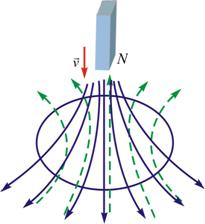
\includegraphics[width=0.9\linewidth]{graphics/楞次定律1.png}
		\caption{磁棒插入导体圆环时}
	\end{subfigure}
	\centering
	\begin{subfigure}{0.25\linewidth}
		\centering
		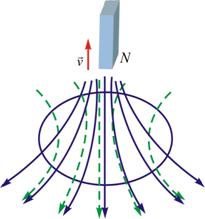
\includegraphics[width=0.9\linewidth]{graphics/楞次定律2.png}
		\caption{磁棒拔出导体圆环时}
	\end{subfigure}
    \caption{楞次定律的应用}
\end{figure}

\subsection{法拉第电磁感应定律}

当通过导体回路的磁通量随时间发生变化时,回路中就有感应电动势产生,从而产生感应电流。这个磁通量的变化可以是由磁场变化引起的,也可以是由于导体在磁场中运动或导体回路中的一部分切割磁力线的运动而产生的。

通过回路所包围面积的磁通量发生变化时,回路中产生的感应电动势 与磁通量对时间的变化率成正比。如果采用国际单位制,则此定律可表示为
\begin{equation}
    \mathscr{E} = - \deriv{\Phi}{t}
\end{equation}
式中的负号时楞次定律的数学表现,或者说我们可以利用式中的负号来确定回路中电磁感应电动势的方向。

如果回路是由\(N\)匝导线串联而成,那么在磁通量变化时,每匝中都将产生感应电动势。如果每匝中通过的磁通量都是相同的,则\(N\)匝线圈中的总电动势应为各匝中电动势的总和,即
\begin{equation}
    \mathscr{E}_i = - N \deriv{\varPhi}{t} = -\deriv{N \varPhi}{t} = -\deriv{\varPsi}{t}
\end{equation}
式中,\(\varPsi = N \varPhi\)称为\emph{磁链}。

如果闭合回路的电阻为\(R\),则回路中的总感应电流为
\begin{equation}
    I_i = \frac{\mathscr{E}}{R} = -\frac{N}{R} \deriv{\varPhi}{t} = -\frac{1}{R} \deriv{\varPsi}{t}
\end{equation}
利用\(I = \dderiv{q}{t}\),可得在\(t_1\)至\(t_2\)时间内通过导线上任一横截面的感应电荷量为
\begin{equation}
    q = \int_{t_1}^{t_2} I_i \rmd t = -\frac{1}{R} \int_{\varPsi_1}^{\varPsi_2} \rmd \varPsi = \frac{1}{R} \left(\varPsi_1 - \varPsi_2\right)= \frac{N}{R} \left(\varPhi_1 - \varPhi_2\right)
\end{equation}

\section{动生电动势}

\emph{动生电动势}是指:导体回路或其一部分在磁场中运动,使其回路面积或回路的法线与磁感应强度B的夹角随时间变化,从而使回路中的磁通量发生变化;

在普遍情况下,一个任意形状的导体线圈\(L\)(不一定闭合)在任意恒定的磁场中运动或发生形变时,\(\rmd L\)和\(v\)的大小和方向都可能是不同的,这时,L中的动生电动势为:
\begin{equation}
    \mathscr{E} = \int \rmd \mathscr{E} = \int_L \left(\boldsymbol{v} \times \boldsymbol{B}\right) \cdot \rmd \boldsymbol{l}
\end{equation}

\section{感生电动势}

当置于磁场中的导体回路不动,而磁场 随时间变化时,也会在导体回路中产生感应电动势,这种感应电动势称为感生电动势。

J.C.Maxwell在分析电磁感应现象的基础上,提出了一个大胆的假设:变化的磁场在其周围空间激发一种新的电场,这种电场是涡旋电场,或称感应电场。产生感生电动势的非静电力就是这个涡旋电场力。

一段导线\(ab\)上的感生电动势为
\begin{equation}
    \mathscr{E}_i = \int \rmd \mathscr{E}_i = \int_{a}^{b} \boldsymbol{E}_i \cdot \rmd \boldsymbol{l}
\end{equation}
对于一个闭合导体回路\(L\),回路内的感生电动势为
\begin{equation}
    \mathscr{E}_i = -\deriv{\varPhi}{t} = \oint_L \boldsymbol{E}_i \cdot \rmd \boldsymbol{l}
    \label{14-7}
\end{equation}
式中\(\varPhi\)是通过闭合回路\(L\)所围成曲面的磁通量。

由于磁通量\(\varPhi = \int_S \boldsymbol{B} \cdot \rmd \boldsymbol{S}\),同时考虑到回路\(L\)及其所围的曲面静止不动,即不随时间变化,代入式\ref{14-7},可得
\begin{equation}
    \oint_L \boldsymbol{E}_i \cdot \rmd \boldsymbol{l} = -\int_{S} \pderiv{\boldsymbol{B}}{t} \cdot \rmd S
    \label{14-8}
\end{equation}
式中\(S\)是以闭合回路\(L\)为周界的任意曲面,曲面\(S\)的法线正方向与回路\(L\)的绕行方向成右手螺旋关系。

静电场的电场线一般起始于正电荷、中指于负电荷,不可能形成闭合曲线。

感生电场是由变化的磁场激发的,与静止电荷无关,它的性质由式\ref{14-8}和下式给出
\begin{equation}
    \oint_S \boldsymbol{E}_i \cdot \rmd \boldsymbol{S} = 0
\end{equation}
即\emph{感生电场是无源的非保守力场},所以感生电场的电场线都是闭合曲线,所以感生电场又称为涡旋电场。

感生电场与静电场唯一的共同点就是对电荷的作用规律相同,即电荷受到的两种电场力钧可以用\(\boldsymbol{F} = q \boldsymbol{E}\)表示。

\subsection{例题}

在半径为\(R\)的圆柱形空间中存在着均匀磁场,磁场方向与圆柱的轴线平行。如图所示,有一长为\(L\)的金属棒放在磁场中,棒的两端恰好在圆周的边缘上。设\(B\)随时间的变化率为\(\dderiv{B}{t}\)。求证:棒上感应电动势的大小为
\begin{equation*}
    \varepsilon=\frac{L}{2} \sqrt{R^2-(L / 2)^2} \deriv{B}{t}
\end{equation*}

\begin{center}
    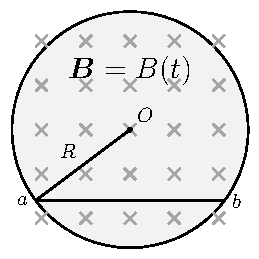
\includegraphics[width=.25\textwidth]{graphics/感生电动势题图.pdf}
\end{center}

\textbf{Solution}

过圆心\(O\) 作金属棒的垂线,垂足为\(O^\prime\),在棒上距\(O^\prime\)为\(x\)处取“棒元”\(\rmd x\),如图所示。

\begin{center}
    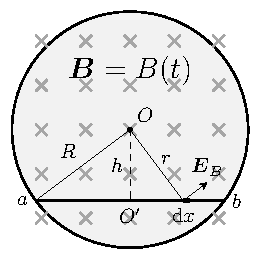
\includegraphics[width=.25\textwidth]{graphics/感生电动势解图.pdf}
\end{center}

由例题,在\(r < R\)的区域,感生电场强度的大小为
\begin{equation*}
    E_B=\frac{r}{2} \frac{\mathrm{~d} B}{\mathrm{~d} t}
\end{equation*}
方向垂直于径向。则该“棒元”上的感生电动势为
\begin{equation*}
\begin{aligned}
& \mathrm{d} \varepsilon=\boldsymbol{E}_B \cdot \mathrm{~d} \boldsymbol{x}=E_B \cos \theta \mathrm{~d} x \\
& =\frac{r}{2} \frac{\mathrm{~d} B}{\mathrm{~d} t} \cdot \frac{h}{r} \cdot \mathrm{~d} x=\frac{h}{2} \frac{\mathrm{~d} B}{\mathrm{~d} t} \mathrm{~d} x
\end{aligned}
\end{equation*}
所以棒ab上的感生电动势的大小为
\begin{equation*}
\begin{gathered}
\varepsilon_{a b}=\int \mathrm{d} \varepsilon=\int_{x_a}^{x_b} \frac{h}{2} \frac{\mathrm{~d} B}{\mathrm{~d} t} \mathrm{~d} x=\frac{1}{2} h \frac{\mathrm{~d} B}{\mathrm{~d} t}\left(x_a-x_b\right)=\frac{1}{2} h L \frac{\mathrm{~d} B}{\mathrm{~d} t} \\
=\frac{L}{2} \sqrt{R^2-(L / 2)^2} \frac{\mathrm{~d} B}{\mathrm{~d} t}
\end{gathered}
\end{equation*}

\section{自感与互感}

\subsection{自感电动势 \quad 自感}

磁链
\begin{equation}
    \varPsi = N \varPhi
\end{equation}

回路通有电流时,该电流产生的磁场会通过回路本身,对于一个确定的线圈,当其通有的电流发生变化时,穿过线圈自身所围面积的磁通量(或磁链)随之发生变化,这时线圈中产生感应电动势的现象称为自感现象。相应的感应电动势称为自感电动势线圈的形状、周围介质(非铁磁性介质)一定时,由毕奥-萨伐尔定律可知,线圈中的电流\(I\)所激发的磁感应强度与\(I\)成正比,\(B \propto I\),故通过线圈自身的磁链更\(\varPsi\)与\(I\)成正比,有
\begin{equation}
    \varPsi = L I
\end{equation}
式中的比例系数L称为自感系数,简称自感,用以描述自感现象的强弱。

回路的自感定义为,回路中的电流为单位值时通过该回路所围面积的磁链数。

\(L\)的数值与线圈的大小、形状、匝数以及其中磁介质的性质有关,即取决于线圈的性质而与线圈中的电流无关。

由法拉第电磁感应定律,线圈中产生的自感电动势为
\begin{equation}
    \mathscr{E}_L = -\deriv{\varPsi}{t} = - L \deriv{I}{t}
\end{equation}

故\(L\)又可定义为:\(L\)的大小等于当电流随时间的变化率为一单位时,回路中产生的自感电动势
\begin{equation}
    L = \frac{\mathscr{E}_L}{-\dderiv{I}{t}}
\end{equation}

\subsection{自感的计算}

对于\(N\)匝线圈组成的回路,若通过每匝线圈的磁感通量都是\(\varPhi\),即每条磁感线交链的电流是每匝中电流的\(N\)倍,那么对整个回路的磁通匝链数为:
\begin{equation}
    \varPsi = N \varPhi
\end{equation}

\begin{figure}[!h]
    \centering
    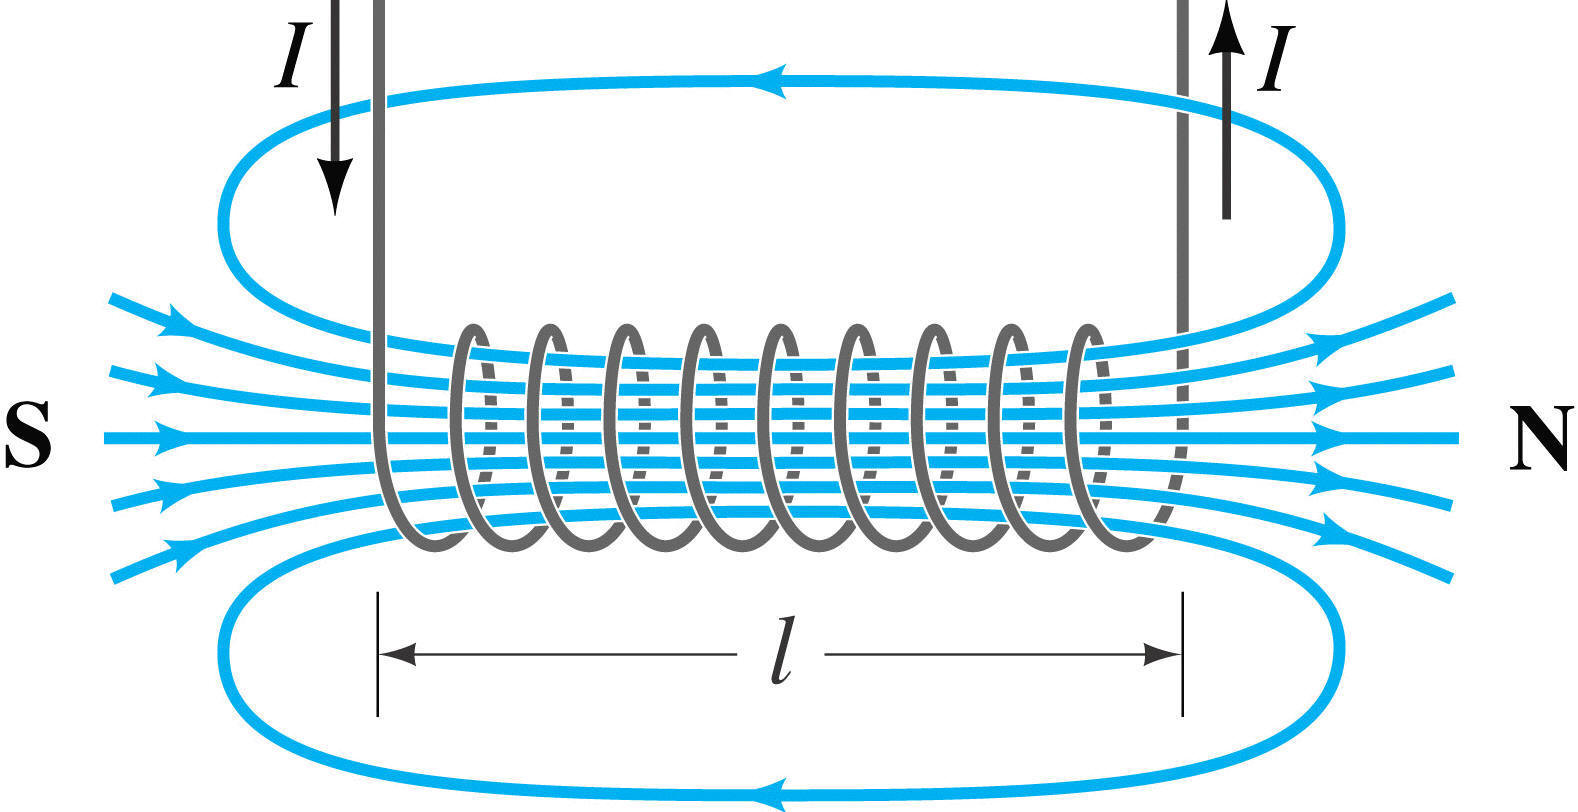
\includegraphics[width = .3\textwidth]{graphics/自感系数的计算.png}
\end{figure}

例如对于理想路线管,横截面积为\(S\),长为\(l\),总匝数\(N\),\(n = \dfrac{N}{l}\),则
\begin{equation}
    \varPsi = N \varPhi = NBS = \mu_0 n^2 I l S
\end{equation}
于是
\begin{equation}
    L = \mu_0 n^2 l S = \mu_0 \frac{N^2}{l^2} V
\end{equation}

\subsubsection{例题}

计算总匝数为N、截面为长方形的螺绕管的自感。

\begin{figure}[!h]
    \centering
    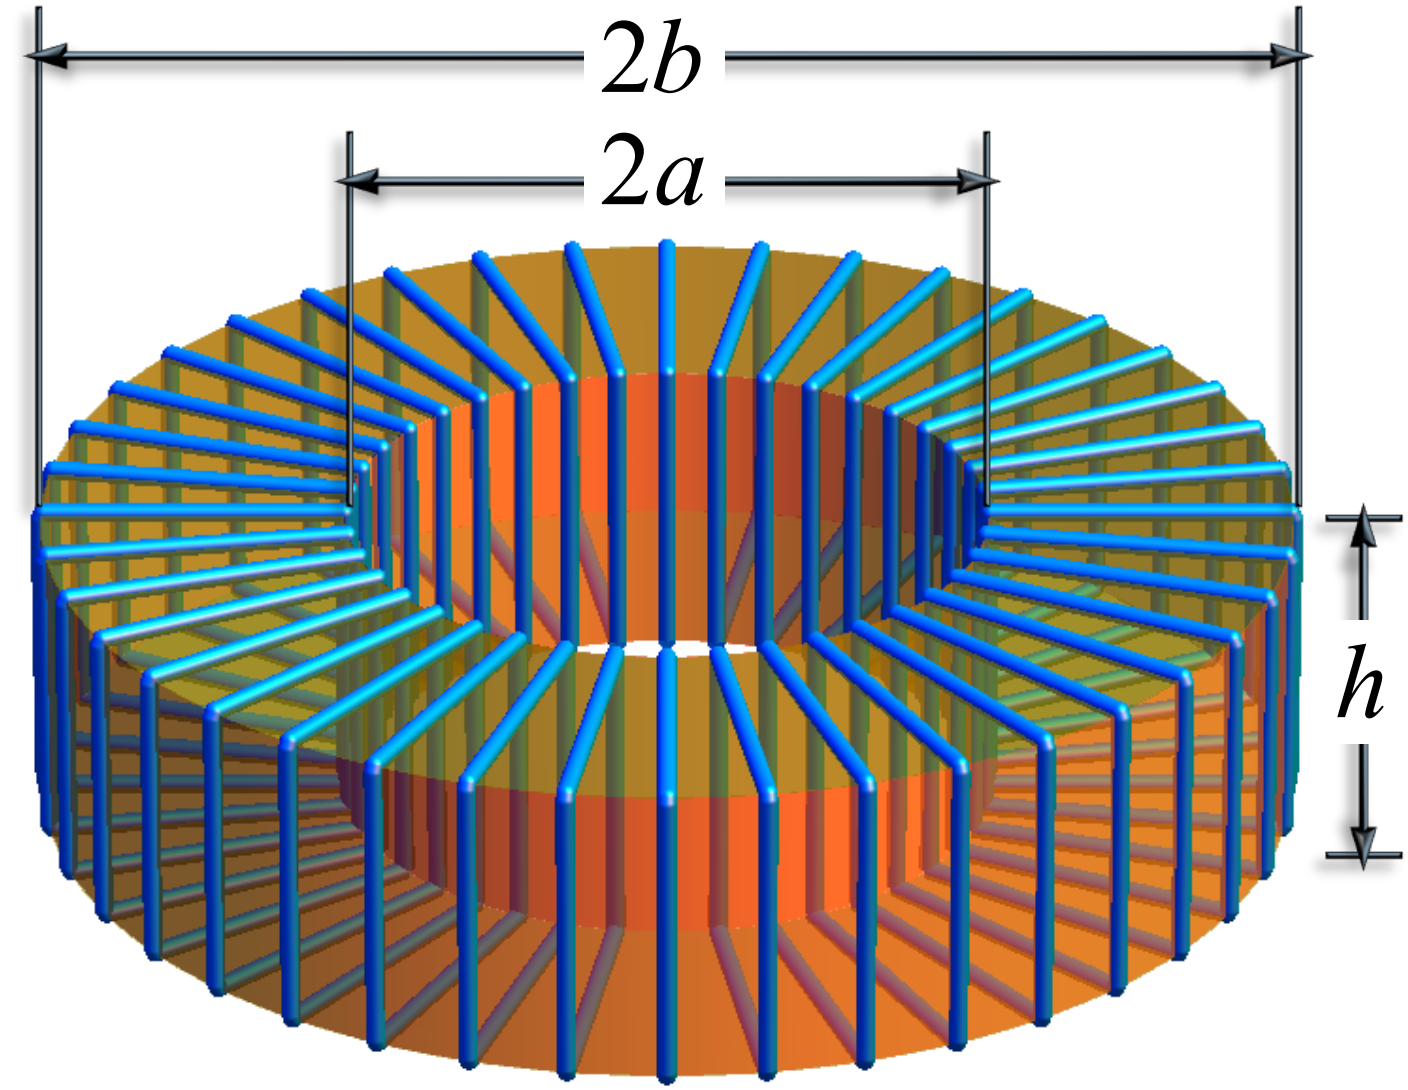
\includegraphics[width = .25\textwidth]{graphics/自感例题.png}
\end{figure}

螺绕管外部磁场为零,内部磁场为
\begin{equation}
    B = \frac{\mu_0 NI}{2\uppi S}
\end{equation}
穿过单匝线圈的磁通量
\begin{equation}
    \varPhi = h \int_{a}^{b} \frac{\mu_0 NI}{2\uppi S} \rmd S = \frac{\mu_0 NIh}{2\uppi} \ln \frac{b}{a}
\end{equation}
自感为
\begin{equation}
    L = \frac{\varPsi}{I} = \frac{\mu_0 N^2 h}{2 \uppi} \ln \frac{b}{a} = \left(2 \times 10^{-7}\right) N^2 h \ln \frac{b}{a}
\end{equation}

\subsection{互感电动势 \quad 互感}

两个相邻导体回路中分别通有电流,当任一载流线圈中的电流发生变化时,周围的磁场随之变化,通过另一个回路所围面积的磁通量也随之变化,因而会在其中产生感应电动势。这种由于一个回路中电流的变化导致在另一个回路中产生感应电动势的现象称为互感现象。相应的感应电动势称为互感电动势。

第一个线圈称为称为初级(主)线圈,第二个称为次级(副)线圈。

\begin{figure}[!h]
    \centering
    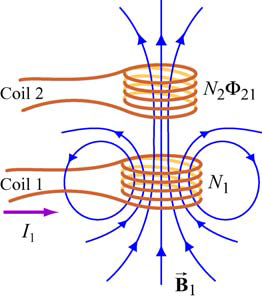
\includegraphics[width = .2\textwidth]{graphics/互感.png}
\end{figure}

线圈1的电流为\(I_1\),它激发的磁场通过线圈2的磁链为\(\varPsi_{21}\),由毕奥-萨伐尔定律知\(I_1\)与\(\varPsi_{21}\)成正比,有
\begin{equation}
    \varPsi_{21} = M_{21} I_1
\end{equation}

线圈1中电流变化时,在线圈2中激发感应电动势为
\begin{equation}
    \mathscr{E}_{21} = - \deriv{\varPsi{21}}{t} = -M_{21} \deriv{I_1}{t}
\end{equation}

\subsection{互感的计算}

\(I_1\)在1中产生的磁场为
\begin{equation}
    B_1 = \mu n_1 I_1 = \mu \frac{N_1}{l} I_1
\end{equation}
由\(I_1\)产生并通过线圈2的磁链为
\begin{equation}
    \varPsi = N_2 B_1 S = \mu \frac{N_1 N_2}{l} S I_1
\end{equation}

互感系数
\begin{equation}
    M = \frac{\varPsi_{21}}{I_1} = \mu \frac{N_1 N_2}{l} S = \mu n_1 n_2 V
\end{equation}

\begin{equation*}
    L_1 = \mu n_1^2 V
\end{equation*}

\begin{equation*}
    L_2 = \mu n_2^2 V
\end{equation*}

\begin{equation}
    M = \sqrt{L_1 L_2}
\end{equation}

一般情况下,由于有存在漏磁
\begin{equation}
    M < \sqrt{L_1 L_2} \text{或} M = k \sqrt{L_1 L_2}
\end{equation}
式中\(k\)为耦合系数,且\(0 \leq k \leq 1\)

\subsection{互感系数的对称性}

\begin{equation*}
    \begin{aligned}
        & \because \overrightarrow{B}_1 = \nabla \times \overrightarrow{A}_1 \\
        & \therefore \varPsi_{21}=\iint_{S_2} \overrightarrow{B}_1 \cdot \rmd \overrightarrow{S}_2=\iint_{S_2}\left(\nabla \times \overrightarrow{A}_1\right) \cdot \rmd \overrightarrow{S}_2=\oint_{C_2} \overrightarrow{A}_1 \cdot \rmd \overrightarrow{l}_2 \\
        & \therefore \overrightarrow{A}_1=\frac{\mu_0}{4 \uppi} \oint_{C_1} \frac{I_1 \rmd \overrightarrow{l}_1}{r_{12}} \\
        & \therefore \varPsi_{21}=\frac{\mu_0 I_1}{4 \uppi} \oint_{C_2} \oint_{C_1} \frac{\rmd \overrightarrow{l}_1 \cdot \rmd \overrightarrow{l}_2}{r_{12}} \\
        & \therefore M_{21}=\frac{\Psi_{21}}{I_1}=\frac{\mu_0}{4 \uppi} \oint_{C_2} \oint_{C_1} \frac{\rmd \vec{l}_1 \cdot \rmd \vec{l}_2}{r_{12}}
    \end{aligned}
\end{equation*}

下标关于1、2交换对称,故有\(M_{21} = N_{12}\)。

\subsubsection{例题}

密绕螺绕管总匝数为\(N\),截面为长方形,几何尺寸如图所示。试求螺绕管与其对称轴上无限长载流直导线的互感系数\(M\)。

\begin{figure}[!h]
    \centering
    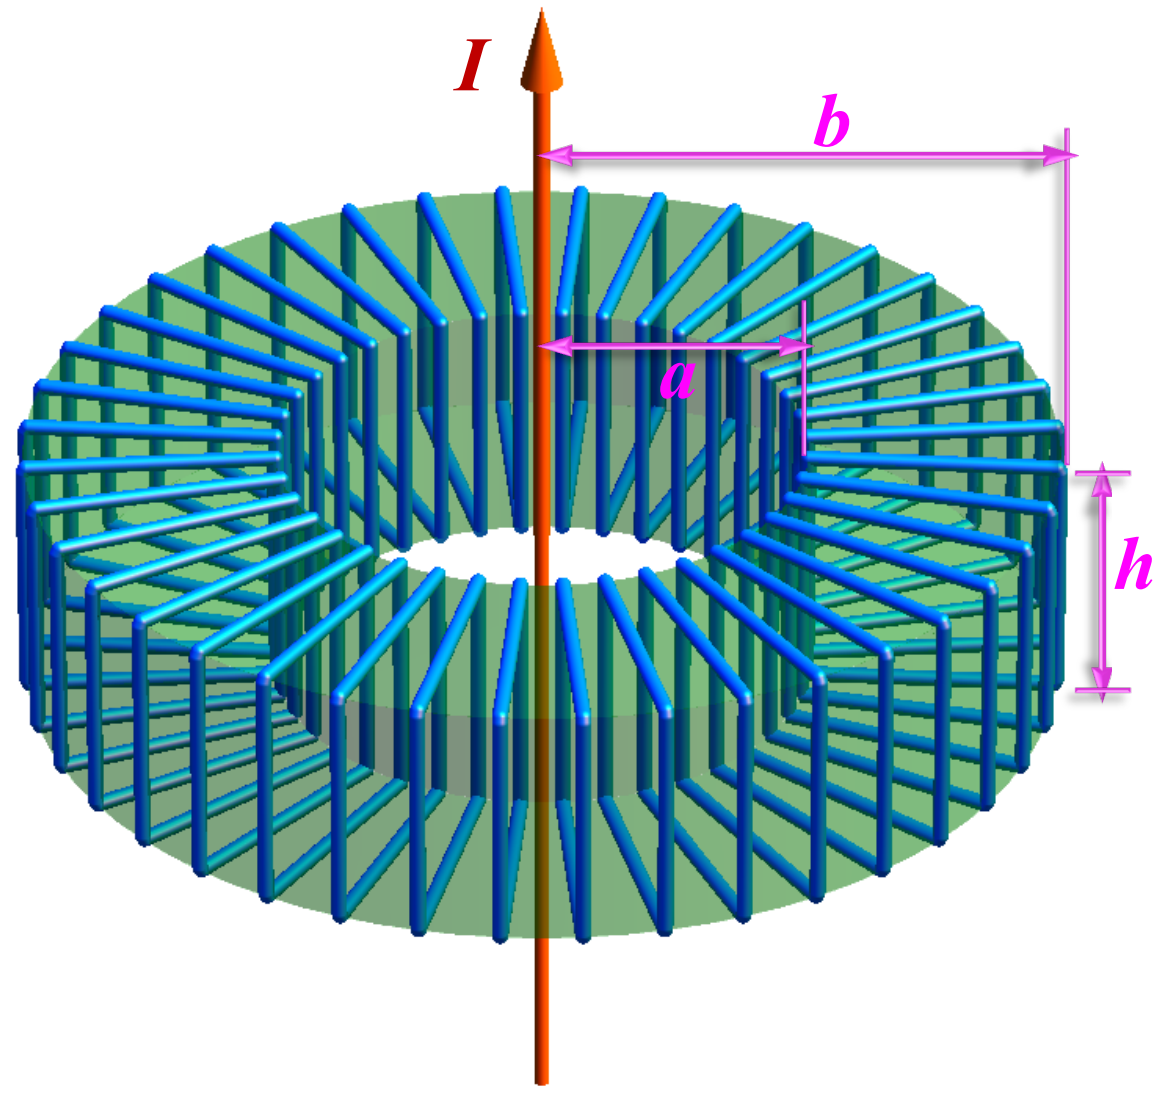
\includegraphics[width = .25\textwidth]{graphics/互感例题.png}
\end{figure}

直导线激发的磁场为
\[
\overrightarrow{B} = \frac{\mu_0 I}{2 \uppi S} \hat{\varPhi}
\]

于是
\begin{equation*}
    \begin{aligned}
        \varPsi &= N \iint_S \overrightarrow{B} \cdot \rmd \overrightarrow{S} \\
        &= \frac{\mu_0 NI}{2 \uppi} \int_{a}^{b} \frac{h \rmd S}{S} \\
        &= \frac{\mu_0 NIh}{2 \uppi} \ln \frac{b}{a}
    \end{aligned}
\end{equation*}
所以
\begin{equation*}
    M = \frac{\varPsi}{I} = \frac{\mu_0 NH}{2 \uppi} \ln \frac{b}{a}
\end{equation*}

\section{磁场的能量}

回路中的自感电动势为\(\mathscr{E}_L = -L\dderiv{i}{t}\),根据欧姆定律\(\mathscr{E} - L \dderiv{i}{t} = i R\),可得电源做的功为
\begin{equation}
    \int_{0}^{\infty} \mathscr{E} i \rmd t = \int_{0}^{\infty} i L\deriv{i}{t} \rmd t + \int_{0}^{\infty} R i^2 \rmd t
\end{equation}
其中$\int_0^{\infty} R i^2 \rmd t$为在电阻上消耗的焦耳热能; $\int_0^{\infty}-i \mathscr{E}_L \rmd t=\int_0^{\infty} i L \deriv{i}{t} \rmd t=\int_0^{I_0} L i \rmd i=\frac{1}{2} L I^2$为电源克服自感电动势而建立恒定磁场所做的功,该功转化成为电感线圈中的能量储存起来,称为磁能或自感磁能,记为
\begin{equation}
W_{\mathrm{m}}=\frac{1}{2} L I^2
\label{14-30}
\end{equation}

考虑长直螺线管的特例,给出磁场能量密度公式。截面积为\(S\)、长为\(l\)、\(N\)匝的长直螺线管,管内充满相对磁导率为\(\mu_0\)的各向同性的均匀磁介质,于是螺线管的自感系数为
$$
L=\mu_0 \mu_r \frac{N^2}{l} S
$$
代入自感磁能公式\ref{14-30},利用\(\mu = \mu_0 \mu_r\),\(B = \mu n I\),得出
\begin{equation}
\begin{aligned}
W_{\mathrm{m}} & =\frac{1}{2} L I^2=\frac{1}{2} \mu \frac{N^2}{l} S I^2 \\
& =\frac{1}{2}\left(\mu \frac{N}{l} I\right)\left(\frac{N}{l} I\right)(S l)=\frac{1}{2} B H V
\end{aligned}
\end{equation}
式中\(V=Sl\)是螺线管的体积,即螺线管内磁场所在空间的体积。那么单位体积磁场的能量,即磁场的能量密度为
\begin{equation}
w_{\mathrm{m}}=\frac{W_{\mathrm{m}}}{V}=\frac{1}{2} B H=\frac{1}{2 \mu} B^2
\label{14-32}
\end{equation}
或用矢量表示,为
\begin{equation}
    w_m = \overrightarrow{B} \cdot \overrightarrow{H}
    \label{14-33}
\end{equation}
公式虽由长直螺线管特例导出但普遍适用。对于非均匀磁场,总的磁场能量为
\begin{equation}
W_{\mathrm{m}}=\int_V w_{\mathrm{m}} \mathrm{~d} V=\int_V \frac{1}{2} \boldsymbol{B} \cdot \boldsymbol{H} \mathrm{~d} V
\label{14-34}
\end{equation}
上式的积分范围为磁场占有的全部空间。式\ref{14-33}和式\ref{14-34}表明,磁场的能量密度和能量完全由描述磁场的矢量\(\overrightarrow{B}\)和\(\overrightarrow{H}\)确定。

\end{document}